\documentclass[12pt]{report}

\usepackage{cmap}
\usepackage[T1,T2A]{fontenc}
\usepackage[utf8]{inputenc}
\usepackage[english, russian]{babel}
\usepackage{amssymb}
\usepackage{amsmath}
\usepackage{amsthm}
\usepackage{dsfont}
\usepackage{bm}
\usepackage{diagbox}
\usepackage[left=20mm,right=10mm,top=20mm,bottom=20mm,bindingoffset=2mm]{geometry}
\usepackage{indentfirst}
\usepackage[utf8]{inputenc}
\usepackage{float}
\usepackage[hidelinks]{hyperref}
\usepackage{graphicx}
\usepackage{xcolor}
\usepackage{listings}
\usepackage{minted}

\DeclareMathOperator{\N}{\mathbb{N}}
\DeclareMathOperator{\R}{\mathbb{R}}
\DeclareMathOperator{\Z}{\mathbb{Z}}
\DeclareMathOperator{\CC}{\mathbb{C}}
\DeclareMathOperator{\PP}{\mathrm{P}}
\DeclareMathOperator{\Expec}{\mathrm{E}}
\DeclareMathOperator{\Var}{\mathrm{Var}}
\DeclareMathOperator{\Cov}{\mathrm{Cov}}
\DeclareMathOperator{\asConv}{\xrightarrow{a.s.}}
\DeclareMathOperator{\LpConv}{\xrightarrow{Lp}}
\DeclareMathOperator{\pConv}{\xrightarrow{p}}
\DeclareMathOperator{\dConv}{\xrightarrow{d}}

\hypersetup{
	colorlinks=true,
	linkcolor=blue,
	citecolor=blue,
	urlcolor=blue
}

\lstset{language=Python, extendedchars=\true}

\lstdefinestyle{pythonstyle}{
	language=Python,
	backgroundcolor=\color{lightgray},
	commentstyle=\color{green},
	keywordstyle=\color{blue},
	stringstyle=\color{red},
	basicstyle=\ttfamily,
	frame=single,
	breaklines=true
}

\begin{document}
	
	\begin{titlepage}
		\begin{center}
			\large{Федеральное государственное автономное образовательное учреждение высшего образования <<Национальный исследовательский университет ИТМО>>}
		\end{center}
		
		\vspace{15em}
		
		\begin{center}
			\huge{\textbf{Курсовая работа}} \\
			\large{По дисциплине <<Информационные системы>>} \\
			\large{Этап №2} \\
		\end{center}
		
		\vspace{5em}
		
		\begin{flushright}
			\textit{\large{Выполнили:}} \\
			\large{Студенты группы P3306} \\
			\large{Михайлов Дмитрий} \\
			\large{Андреевич} \\
			\large{Медведев Владислав} \\
			\large{Александрович} \\
			\textit{\large{Преподаватель:}} \\
			\large{Коновалов Арсений} \\
			\large{Антонович}
		\end{flushright}
		
		\vspace{2cm}
		
		\begin{figure}[h]
			\centering
			
\includegraphics[width=0.5\linewidth]{image.png}
		\end{figure}
		
		\begin{center}
			Санкт-Петербург \\
			2025 год
		\end{center}
	\end{titlepage}
	
	\tableofcontents
	\newpage
	
	\addcontentsline{toc}{section}{Задание}
	\section*{Задание}
	\begin{enumerate}
		\item Сформировать ER-модель базы данных (на основе описаний предметной области и прецедентов из предыдущего этапа). ER-модель должна:
		\begin{itemize}
			\item[a.] включать не менее десяти сущностей;
			\item[b.] содержать хотя бы одно отношение вида «многие-ко-мндным» (m:N).
		\end{itemize}
		
		\item Согласовать ER-модель с преподавателем. \\
		
		\item На основе ER-модели построить даталогическую модель. \\
		
		\item Реализовать даталогическую модель в реляционной СУБД PostgreSQL. \\
		
		\item Обеспечить целостность данных при помощи средств языка DDL и триггеров. \\
		
		\item Реализовать скрипты для создания базы данных, удаления базы данных, заполнения базы тестовыми данными. \\
		
		\item Предложить pl/pgsql-функции и процедуры для выполнения критически важных запросов (которые потребуются при последующей реализации прецедентов). \\
		
		\item Создать индексы на основе анализа использования базы данных в контексте описанных на первом этапе прецедентов. Обосновать полезность созданных индексов для реализации бизнес-процессов, описанных на первом этапе. \\
		
		\item Составить отчет. \\
	\end{enumerate}
	\newpage
	
	\addcontentsline{toc}{section}{ER-model}
	\section*{ER-model}
	
	\begin{figure}[h]
		\centering
		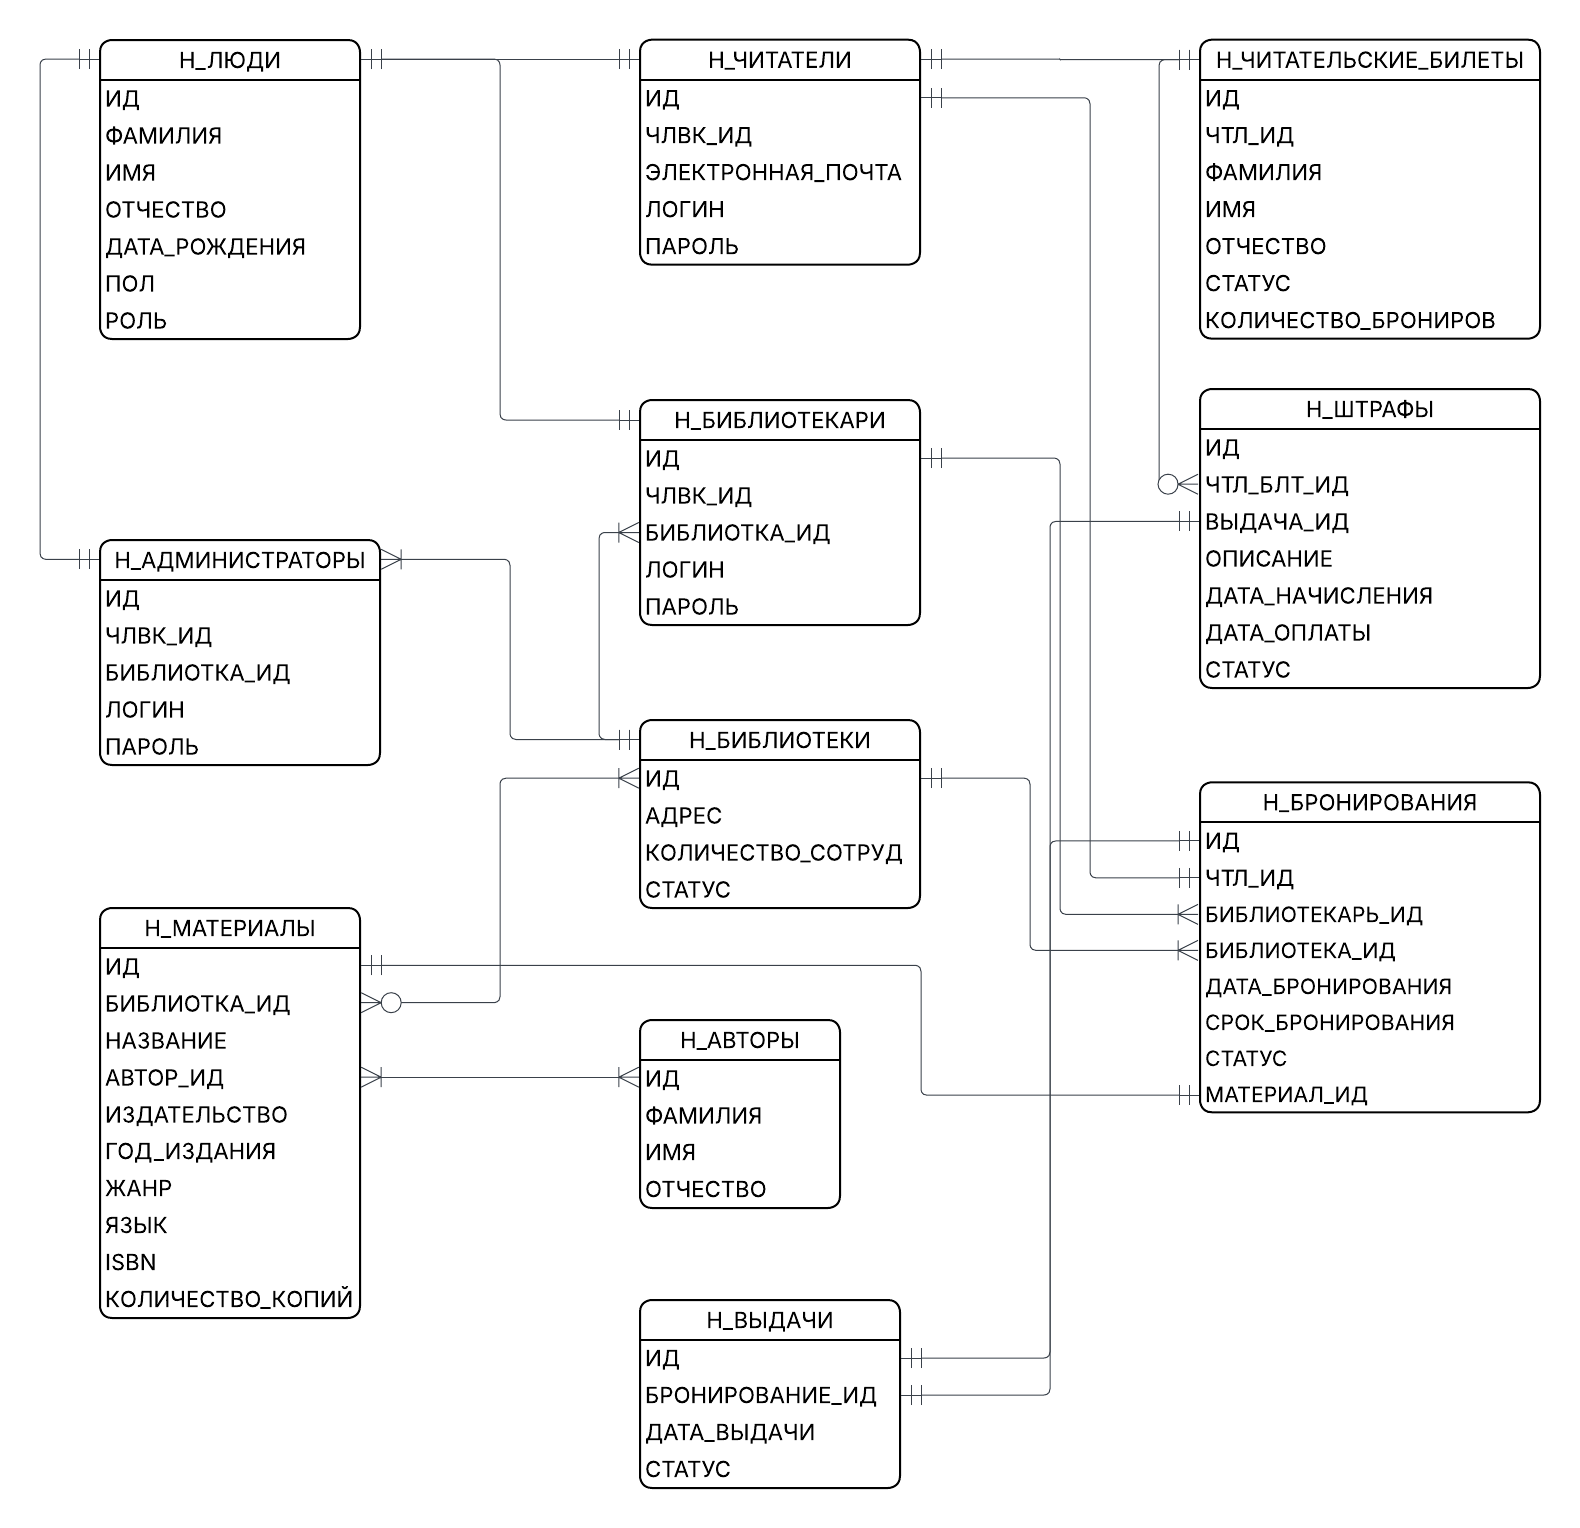
\includegraphics[width=0.8\textwidth]{ER-model.png}
		\caption{ER-модель на основе описаний предметной области и прецедентов из предыдущего этапа.}
		\label{fig:ER-model}
	\end{figure}
	\newpage
	
	\addcontentsline{toc}{section}{Даталогическая модель}
	\section*{Даталогическая модель}
	
	\begin{figure}[h]
		\centering
		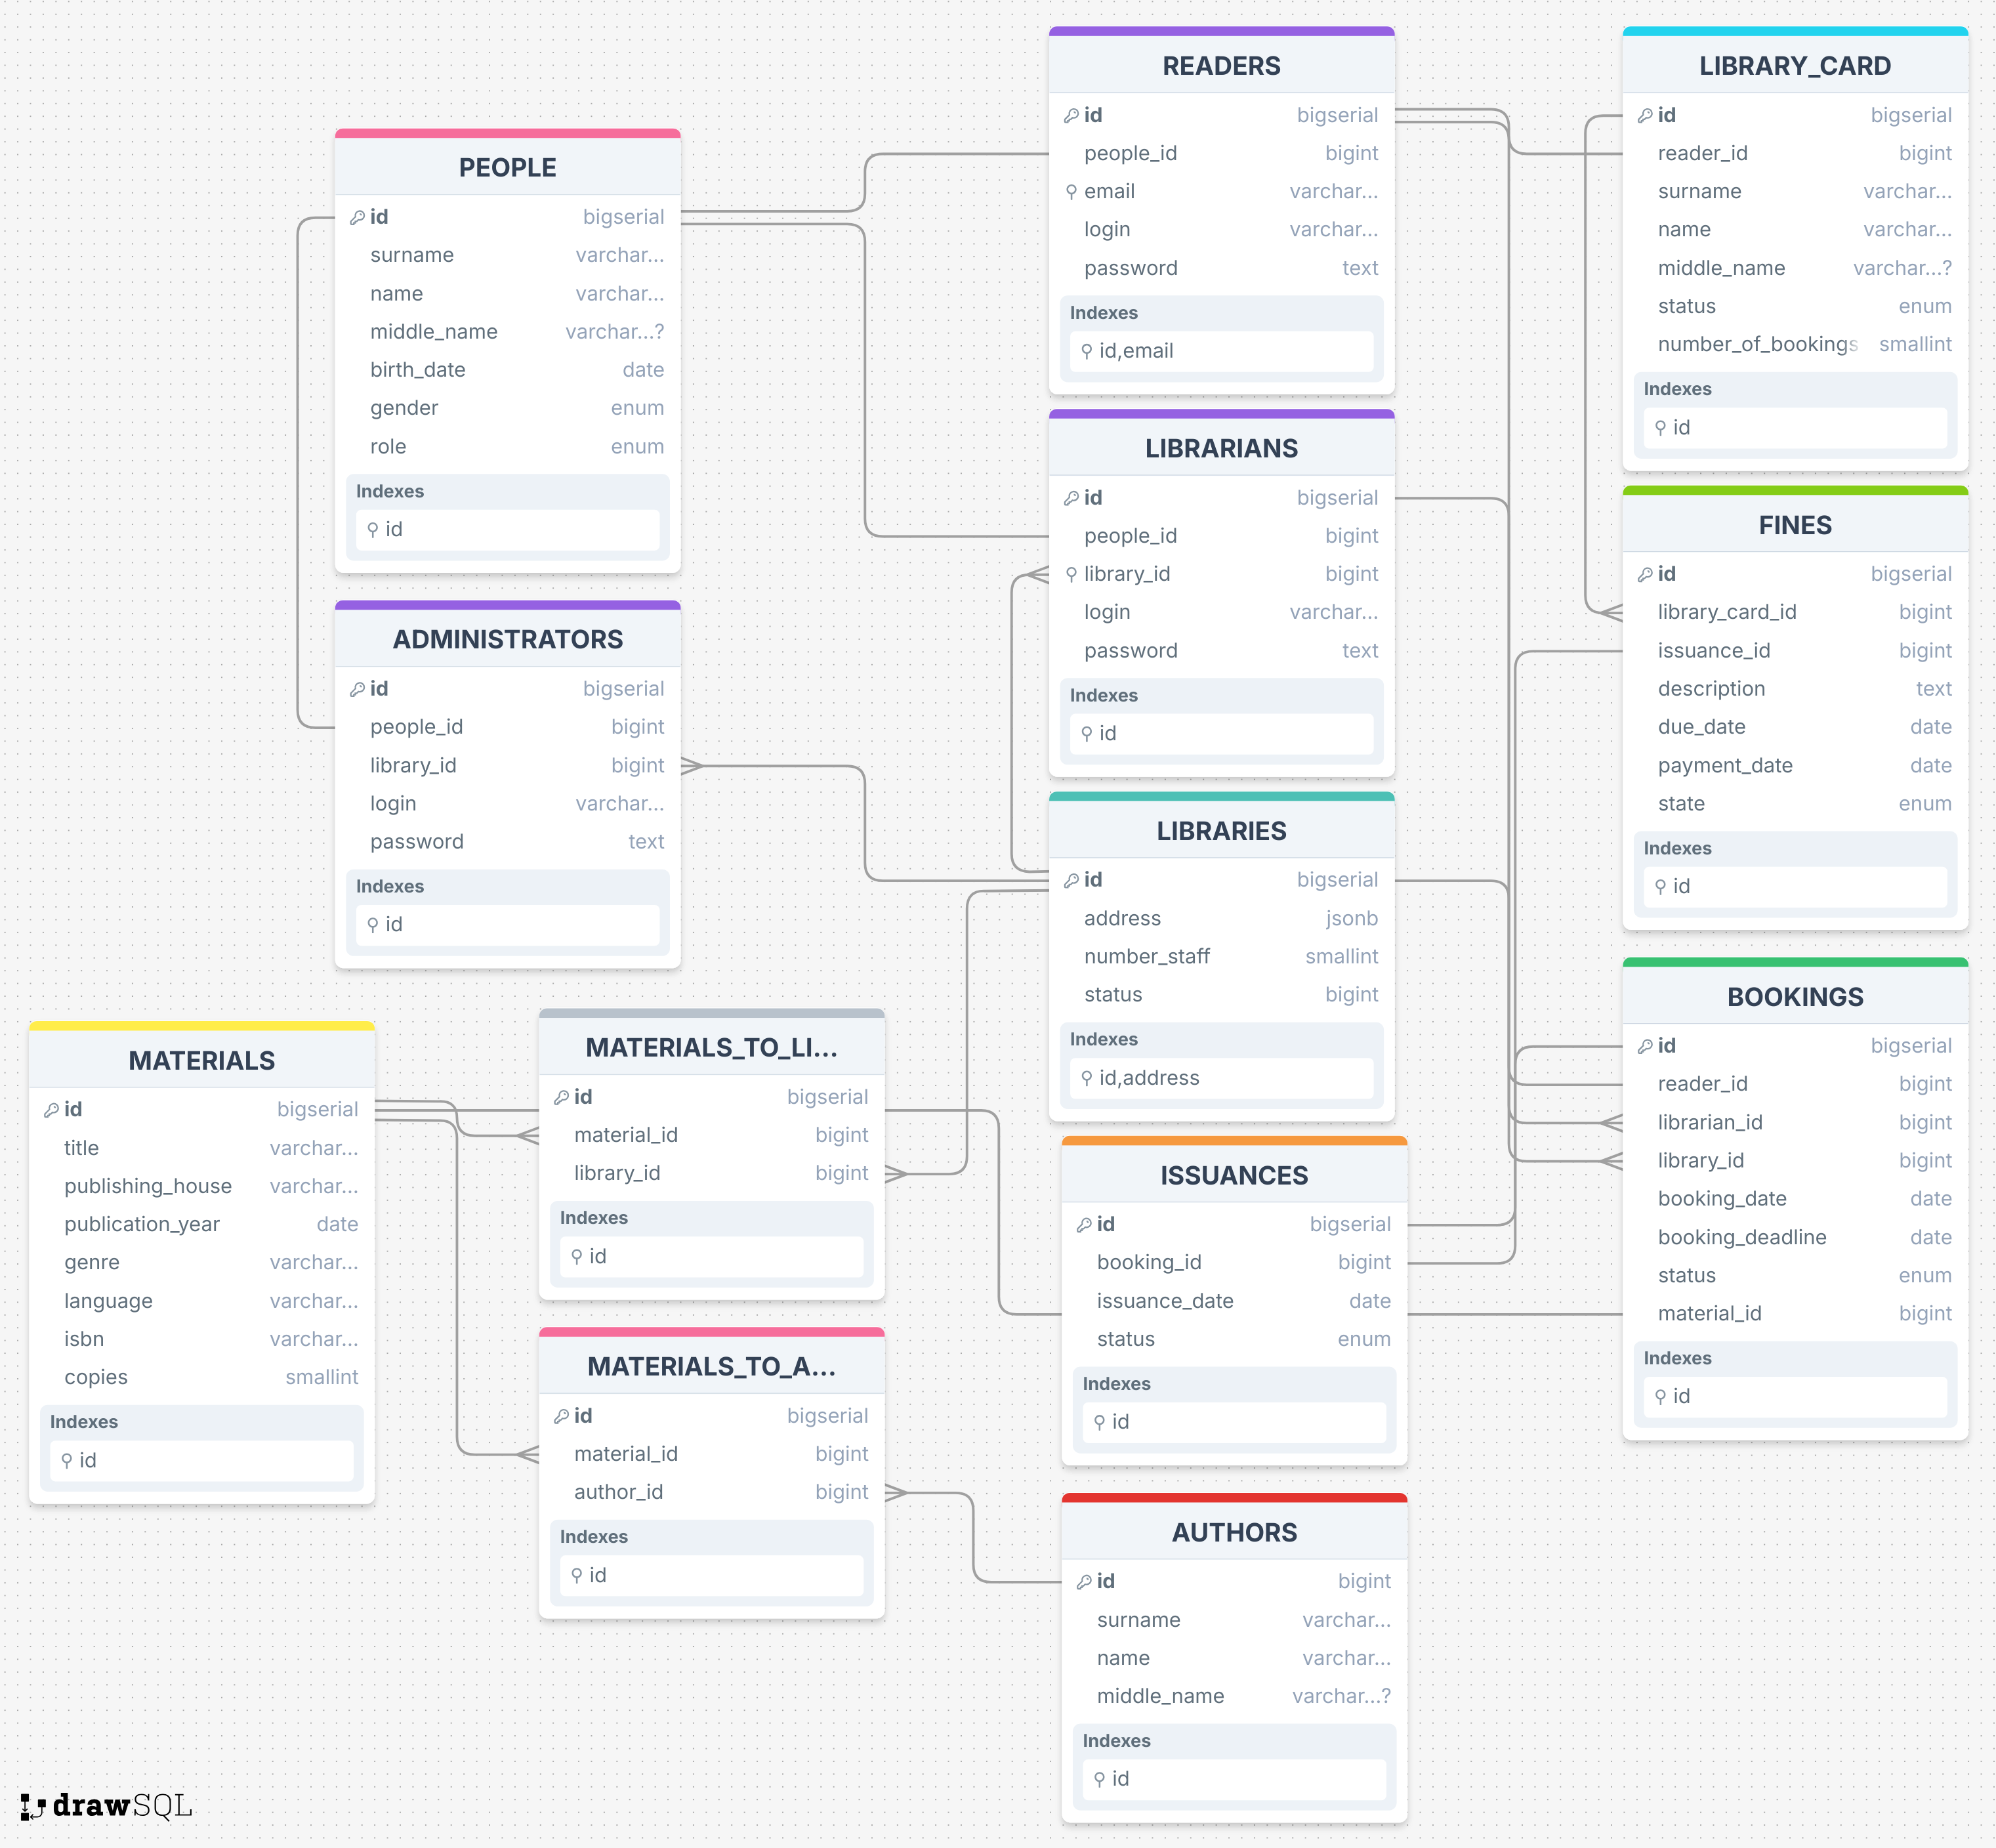
\includegraphics[width=1\textwidth]{Logical-Data-Model.png}
		\caption{Даталогическая модель на основе ER-модели.}
		\label{fig:Logical data model}
	\end{figure}
	\newpage
	
	
	\addcontentsline{toc}{section}{Листинг программы}
	\section*{Листинг программы}
	\href{https://github.com/mysticslippers/information_systems_archive/tree/main/%D0%A1ourse_work/%D0%9A%D1%83%D1%80%D1%81%D0%BE%D0%B2%D0%B0%D1%8F%20%D1%80%D0%B0%D0%B1%D0%BE%D1%82%D0%B0%2C%20%D0%AD%D1%82%D0%B0%D0%BF%20%E2%84%962/code}{Ссылка на репозиторий с кодом.}
	
\end{document}
